
% =================================================================================
%===================================================================================
%===================================================================================
%===================================================================================
% CORREGIR LAPSOS DE TIEMPO EN GANTT Y TABLA DE CALCULO DE HORAS INVERTIDAD CON RESPECTO AL LAPSO CONTEMPLADO EN FACTIBILIDAD DESARROLLADO POR REBECA. Hacer concordar el labso total de tiempo de trabajo. 
%===================================================================================
%===================================================================================
%===================================================================================
%===================================================================================
%===================================================================================
%===================================================================================




La factibilidad operativa se refiere a la evaluación para determinar si un equipo de trabajo u organización dispone de los suficientes recursos humanos y productivos para la realización de un proyecto determinado. 

En este apartado se describren los perfiles de conocimientos necesarios dentro del equipo de trabajo así como las funciones del personal durante el trabajo. El desarrollo de factibilidad operativa en el contexto de este Trabajo Terminal, consiste en determinar el grado de viabilidad para que los peatones de la alcaldía Gustavo A. Madero adopten y utilicen el prototipo de aplicación móvil en su rutina diaria de movilidad.

Para garantizar que el sistema sea operativamente viable, se analizan los siguientes factores clave:

\begin{itemize}
    \item \textbf{Perfil de conocimientos dentro del equipo y roles de trabajo}
    \item\textbf{Procesos y flujos de trabajo}
    \item \textbf{Factibilidad temporal}
\end{itemize}

\subsubsection{Perfil de conocimientos dentro del equipo y roles de trabajo}

En la tabla \ref{tab:conoc_generales} se muestran a detalle los conocimientos generales necesarios de los que deben disponer todos los integrantes del equipo para desarrollar el trabajo en optimas condiciones con el objetivo de asegurar el completo entendimiento de las herramientas, aplicaciones o temas involucrados con el sistema. 

\begin{table}[H]
\centering
\scriptsize
\renewcommand{\arraystretch}{1.5}
\begin{tabular}{| >{\centering\arraybackslash}m{0.5\textwidth} | c |}
\hline
\textbf{Conocimientos técnicos generales necesarios para el desarrollo del proyecto} & \textbf{¿El equipo cumple el requisito?} \\ \hline
Experiencia en el manejo de Entornos de Desarrollo Integrado (IDE) y editores de código. & Sí \\ \hline
Manejo de lenguajes de desarrollo relacionados con el entorno de aplicaciones móviles & Sí \\ \hline
Conocimiento en Base de datos y diagramado & Sí \\ \hline
Comprensión general del funcionamiento de algoritmos para problemas SPP y nociones de lógica algorítmica & Sí \\ \hline
Experiencia en diseño y desarrollo UI/UX & Sí \\ \hline
Conocimientos generales en desarrollo Front-End y Back-End & Sí \\ \hline
Gestión ágil de proyectos de software y manejo de sistemas de control de versiones & Sí \\ \hline

\end{tabular}
\caption{Evaluación de conocimientos generales del equipo}
\label{tab:conoc_generales}
\end{table}

Como se puede apreciar en la tabla \ref{tab:conoc_generales} se determina que el equipo cumple con los conocimiento iniciales necesarios para llevar a cabo el proyecto. Se toma como base el perfil básico de un ingeniero en sistemas computacionales considerando que los tres integrantes del equipo están actualmente cursando la carrera de Ingeniería en Sistemas Computacionales (2020) dentro de la Escuela Superior de Computo del IPN (Instituto Politécnico Nacional) y se encuentran en sus últimos semestres.

La definición de roles se realizo previamente dentro de la sección \ref{Roles_equip}. A continuación la tabla \ref{tab:roles_conocimientos} muestra la descripción general de los roles establecidos en la metodología de desarrollo Scrumban y los conocimientos requeridos para el desarrollo del TT. 

\begin{table}[H]
\centering
\scriptsize
\renewcommand{\arraystretch}{1.5}
\begin{tabular}{| >{\centering\arraybackslash}m{0.15\textwidth} | >{\centering\arraybackslash}m{0.20\textwidth} | >{\centering\arraybackslash}m{0.40\textwidth} | >{\centering\arraybackslash}m{0.15\textwidth} |}
\hline
\textbf{Rol} & \textbf{Asignación} & \textbf{Conocimientos específicos requeridos} & \textbf{Nivel de dominio} \\ \hline

\textbf{Scrum Master} & Rebeca Hernández Simón & Gestión de marcos de trabajo ágiles (Scrumban), administración de tableros Kanban, métricas de esfuerzo y resolución de bloqueos operativos. & Alto (85\%) \\ \hline

\textbf{\textit{Product Owner}} & Fernando Mendoza Segura & Ingeniería de requerimientos, priorización del \textit{Product Backlog} y visión integral de la arquitectura del sistema (base de datos, lógica algorítmica y \textit{frontend}). & Intermedio (60\%) \\ \hline

\textbf{Líder de QA} & Alan Ivan Sánchez Gómez & Diseño de interfaces (UI), evaluación heurística de experiencia de usuario (UX), diseño de casos de prueba y ejecución de pruebas de integración. & Avanzado (90\%) \\ \hline

\textbf{Equipo de desarrollo} & Todos los integrantes & Programación de aplicaciones móviles (Dart/Flutter), administración de bases de datos espaciales (PostGIS/pgRouting), algoritmos de ruteo y control de versiones (Git). & Alto (80\%) \\ \hline
\end{tabular}
\caption{Distribución de roles, conocimientos y nivel de dominio del equipo}
\label{tab:roles_conocimientos}
\end{table}

Para cuantificar el nivel de dominio de los conocimientos específicos requeridos por el equipo de desarrollo y justificar la factibilidad operativa del proyecto, se establece la siguiente métrica de evaluación basada en rangos porcentuales:

\begin{itemize}
    \item \textbf{Bajo (0\% - 40\%):} Conocimiento teórico elemental o nulo. 
    \item \textbf{Intermedio (41\% - 60\%):} Conocimiento funcional y práctico. 
    \item \textbf{Alto (61\% - 80\%):} Dominio sólido y autónomo. 
    \item \textbf{Avanzado (81\% - 100\%):} Experiencia técnica superior y capacidad de liderazgo. 
\end{itemize}

La determinación del nivel de dominio en la tabla \ref{tab:roles_conocimientos} se realizo con base a una autoevaluación de experiencia practica en el manejo de los conocimientos declarados en la tabla de roles.

\textbf{Nota}: Es importante mencionar que pese a que hay una distribución de roles que señala cuales conocimientos deben ser manejados por ciertos integrantes en especifico, como el equipo de desarrollo esta compuesto por todos los miembros, cada uno debe tener familiarización con la mayoría de los conocimientos requeridos en general, para segurar el entendimiento del sistema y facilitar el apoyo entre procesos de trabajo y tareas que se lleguen a dificultar.

\subsubsection{Procesos y flujos de trabajo}

En este apartado se analiza como es que el sistema y las actividades o trabajos relacionados a su desarrollo se integran en los flujos de trabajo evitando detener operaciones del negocio, del equipo o del desarrollo. 

Considerando que el trabajo se realiza siguiendo los esquemas de trabajo, metodologias , datos, enfoques y variables desarrolladas en el capitulo \ref{cap:marco_metodologico}, es de donde directamente se tomaran los procesos de trabajo para el estudio de factibilidad operativa. 

La metodología de desarrollo para el proyecto es Scrumban la cual funciona como marco de gestión general para todo el desarrollo del proyecto mientras que en la fase de programación es integran esquemas de trabajo propios de otras dos metodologías: Incremental y Prototipos. 

En la tabla \ref{tab:proc_trabajo} se definen a detalle los procesos y flujo de trabajo relacionados al marco metodológico, centrándose en el seguimiento del proyecto con base a las metodologías seleccionadas para la gestión y el desarrollo de la aplicación móvil con la finalidad de determinar si dichos procesos afectan de forma positiva o negativa en la factibilidad operativa. 

\begin{table}[H]
\centering
\scriptsize
\renewcommand{\arraystretch}{2} 
\begin{tabular}{| p{0.3\textwidth} | p{0.1\textwidth} | p{0.5\textwidth} |}
\hline
\textbf{Ámbitos laborales} & \textbf{ID} & \textbf{Proceso o flujo de trabajo definido} \\ \hline

\multirow{4}{=}{Marco de gestión: Scrumban, y Documentación} 
& S-1 & El seguimiento del proyecto y actividades establecidas se realiza por medio de reuniones semanales donde se proporciona retroalimentación de los avances entre todos los integrantes.  \\ \cline{2-3}
& S-2 & La organización de actividades y pendientes se realiza mediante un tablero Kanban que se actualiza según las necesidades del equipo. \\ \cline{2-3} 
& S-3 & El equipo dedica 10 a 20 horas mínimas a la semana para el desarrollo de la documentación a través de un proyecto compartido en Overleaf. \\ \cline{2-3} 
& S-4 & La priorización del \textit{Product Backlog} se realiza al inicio de cada iteración para enfocar el esfuerzo de programación en los requerimientos más críticos. \\ \hline 

\multirow{5}{=}{Fase de desarrollo del prototipo} 
& F-1 & El desarrollo del sistema se divide en módulos funcionales independientes. La integración validada de cada módulo a la rama principal del código constituye un nuevo incremento del producto. \\ \cline{2-3} 
& F-2 & Cada incremento en el sistema parte como un prototipo para observar el valor que proporciona y la dificultad de su desarrollo formal para decidir si continuar con el incremento, descartarlo, pausarlo o re-asignarle una nueva prioridad. \\ \cline{2-3} 
& F-3 & El código fuente se gestiona de manera centralizada en GitHub, utilizando ramas independientes para desarrollar cada nueva característica de forma aislada. \\ \cline{2-3}
& F-4 & Antes de integrar cualquier avance a la rama principal, se realiza una revisión cruzada para evitar conflictos y asegurar la estabilidad. \\ \cline{2-3}
& F-5 & La codificación se distribuye según las fortalezas técnicas (Flutter, PostGIS, ruteo), pero se mantiene una arquitectura compartida para que todos conozcan el sistema. \\ \hline

\multirow{2}{=}{Diseño de Interfaces y Experiencia de Usuario (UI/UX)}
& U-1 & Previo a la codificación en el \textit{framework} móvil, se diseñan maquetas (mockups) interactivas para validar la navegación y ubicación de los elementos visuales. \\ \hline

\end{tabular}
\caption{Procesos y flujos de trabajo dividos en ámbitos laborales}
\label{tab:proc_trabajo}
\end{table}

\begin{table}[H]
\centering
\scriptsize
\renewcommand{\arraystretch}{2} 
\begin{tabular}{| p{0.3\textwidth} | p{0.1\textwidth} | p{0.5\textwidth} |}
\hline
\textbf{Ámbitos laborales} & \textbf{ID} & \textbf{Proceso o flujo de trabajo definido} \\ \hline

\multirow{3}{=}{Control de calidad (QA) y Pruebas.} 
& Q-1 & El Líder de QA ejecuta pruebas de integración y valida la usabilidad de las interfaces antes de dar por finalizado y aprobado cada incremento del prototipo. \\ \cline{2-3}
& Q-2 & Los errores técnicos identificados (\textit{bugs}) se registran inmediatamente en el tablero de trabajo para ser resueltos antes de avanzar a la siguiente fase. \\ \cline{2-3}
& Q-3 & Se evalúa el rendimiento del sistema mediante pruebas de latencia para garantizar que el cálculo de rutas seguras no exceda los tiempos de respuesta operativos. \\ \hline


\multirow{3}{=}{Seguimiento e interacciones con los evaluadores interesados en el proyecto} 
& I-1 & El seguimiento del trabajo con las partes interesadas en el, se llevan a cabo mediante reuniones presenciales donde se presentan los avances del producto y se hacen retroalimentaciones.\\ \cline{2-3} 
& I-2 & El número de reuniones al igual que la fecha lo definen los evaluadores y el equipo busca adaptarse a estas necesidades.  \\ \cline{2-3} 
& I-3 & A las correcciones señaladas por el grupo de interesados en el proyecto se les dará prioridad con el objetivo de presentar un avance satisfactorio en la siguiente reunión o revisión.  \\ \hline

\end{tabular}
\caption*{Continuación de la tabla \ref{tab:proc_trabajo}}
\end{table}

Como se muestra en la tabla \ref{tab:proc_trabajo}, la integración del sistema es operativamente factible. Los procesos definidos no interrumpen las actividades habituales del equipo, sino que optimizan su flujo de trabajo continuo durante el desarrollo.

\subsubsection{Factibilidad Temporal}

Se ha comprobado que el personal esta capacitado para la elaboración del TT y que los procesos definidos son adecuados para no interferir con las operaciones diarias de trabajo por lo que ahora toca analizar si el tiempo establecido para desarrollar el producto es adecuado respecto a las fechas laborales y cantidad de horas invertidas. Cabe mencionar que también se comprueba si el personal disponible tiene la capacidad de cubrir totalmente la elaboración del proyecto según los tiempos establecidos. 

El análisis de factibilidad temporal entra como un sub apartado de factibilidad operativa ya que solamente requiere enfocarse en el análisis de operaciones y distribución de tareas conforme al plazo establecido, es decir, se analiza si es posible realizar el proyecto dentro del tiempo definido. 

En el Diagrama de Gantt \ref{fig:cronograma_actividades} se muestra la definición de trabajos para todo el desarrollo del trabajo terminal partiendo desde la fase inicial de investigación y finalizando hasta la entrega del prototipo de aplicación móvil completamente funcional junto con la documentación terminada por completo. 

\begin{figure}[H]
    \centering
    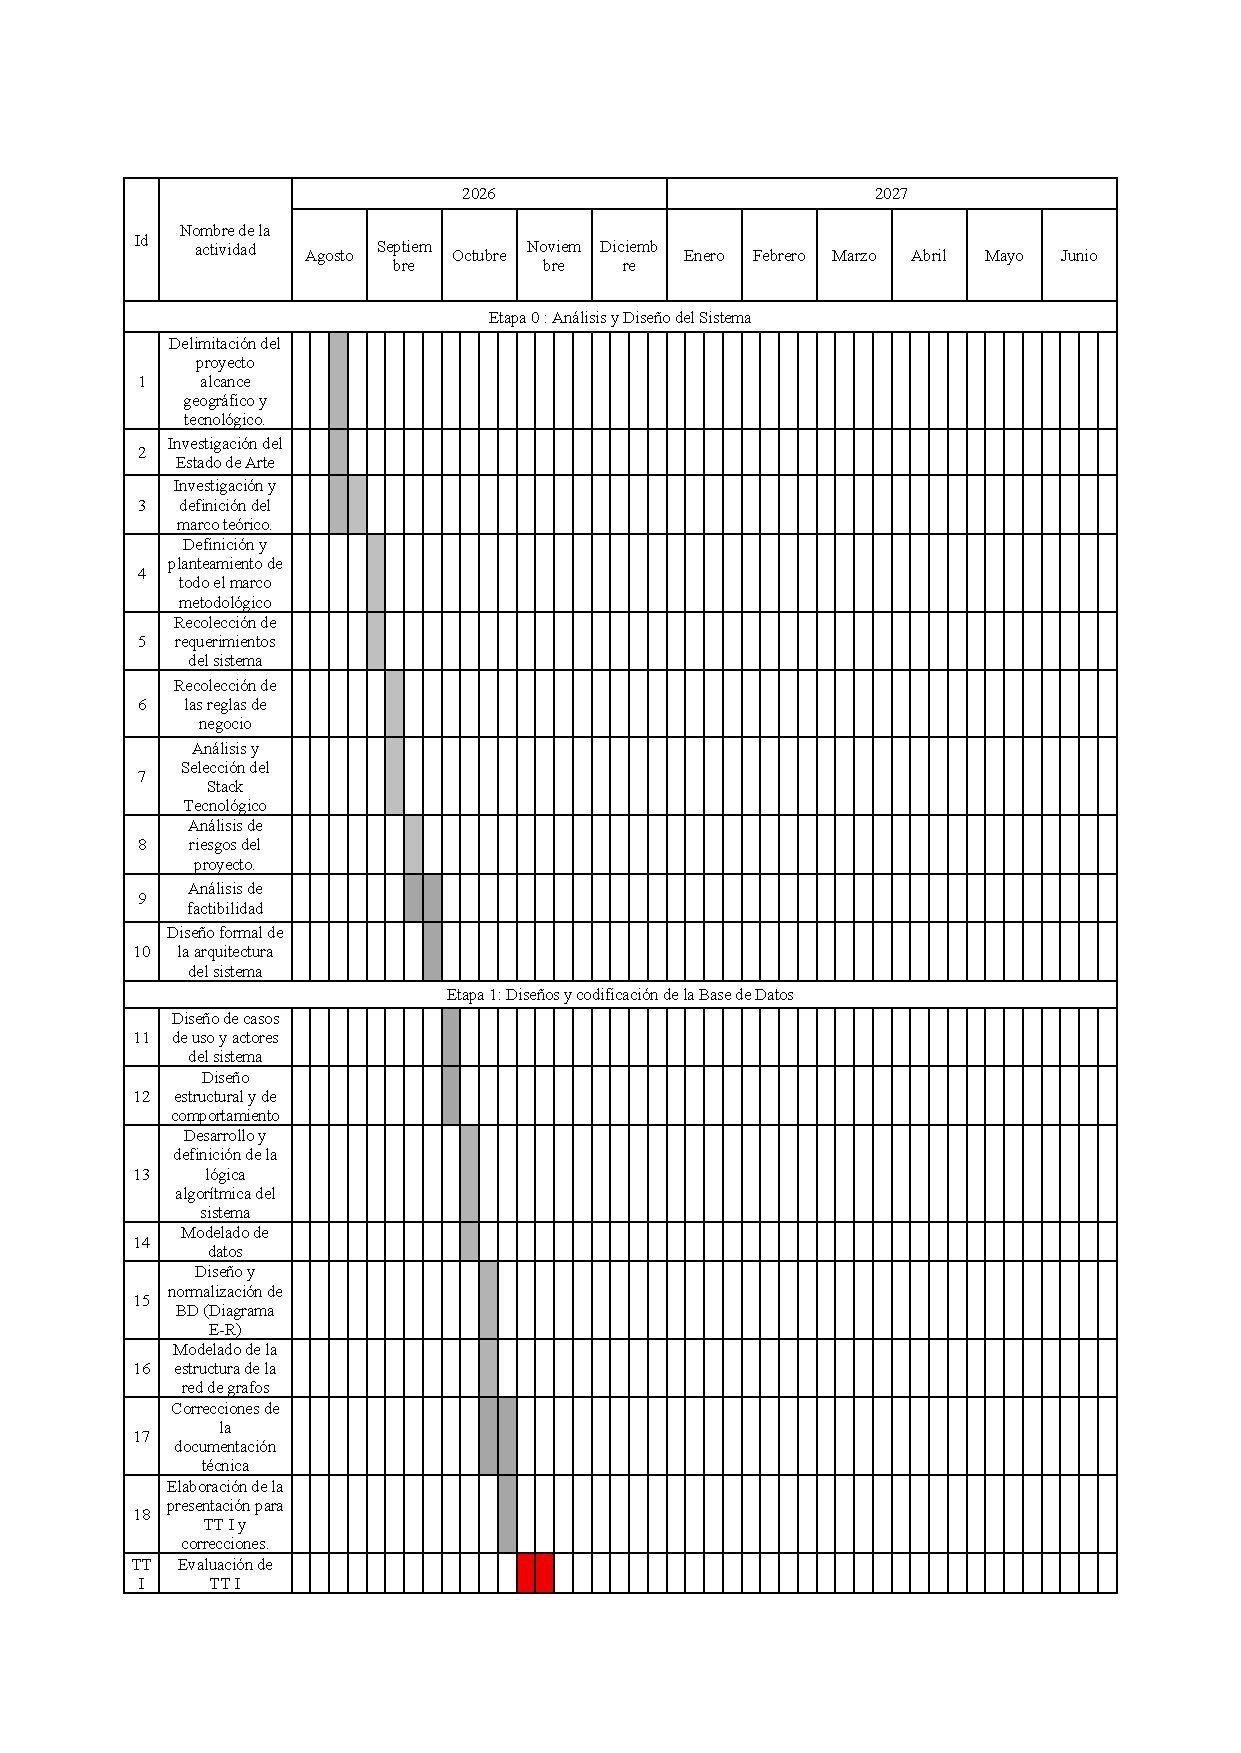
\includegraphics[width=\textwidth, trim={2cm 2cm 2cm 3cm}, clip]{figures/capitulo5_analisis_sistema/5.5_Analisis_de_Factibilidad/Cronograma_2027_TT1.pdf} 
    \caption{Diagrama de Gantt general de actividades del Trabajo Terminal}
    \label{fig:cronograma_actividades}
\end{figure}

\begin{figure}[H]
    \centering
    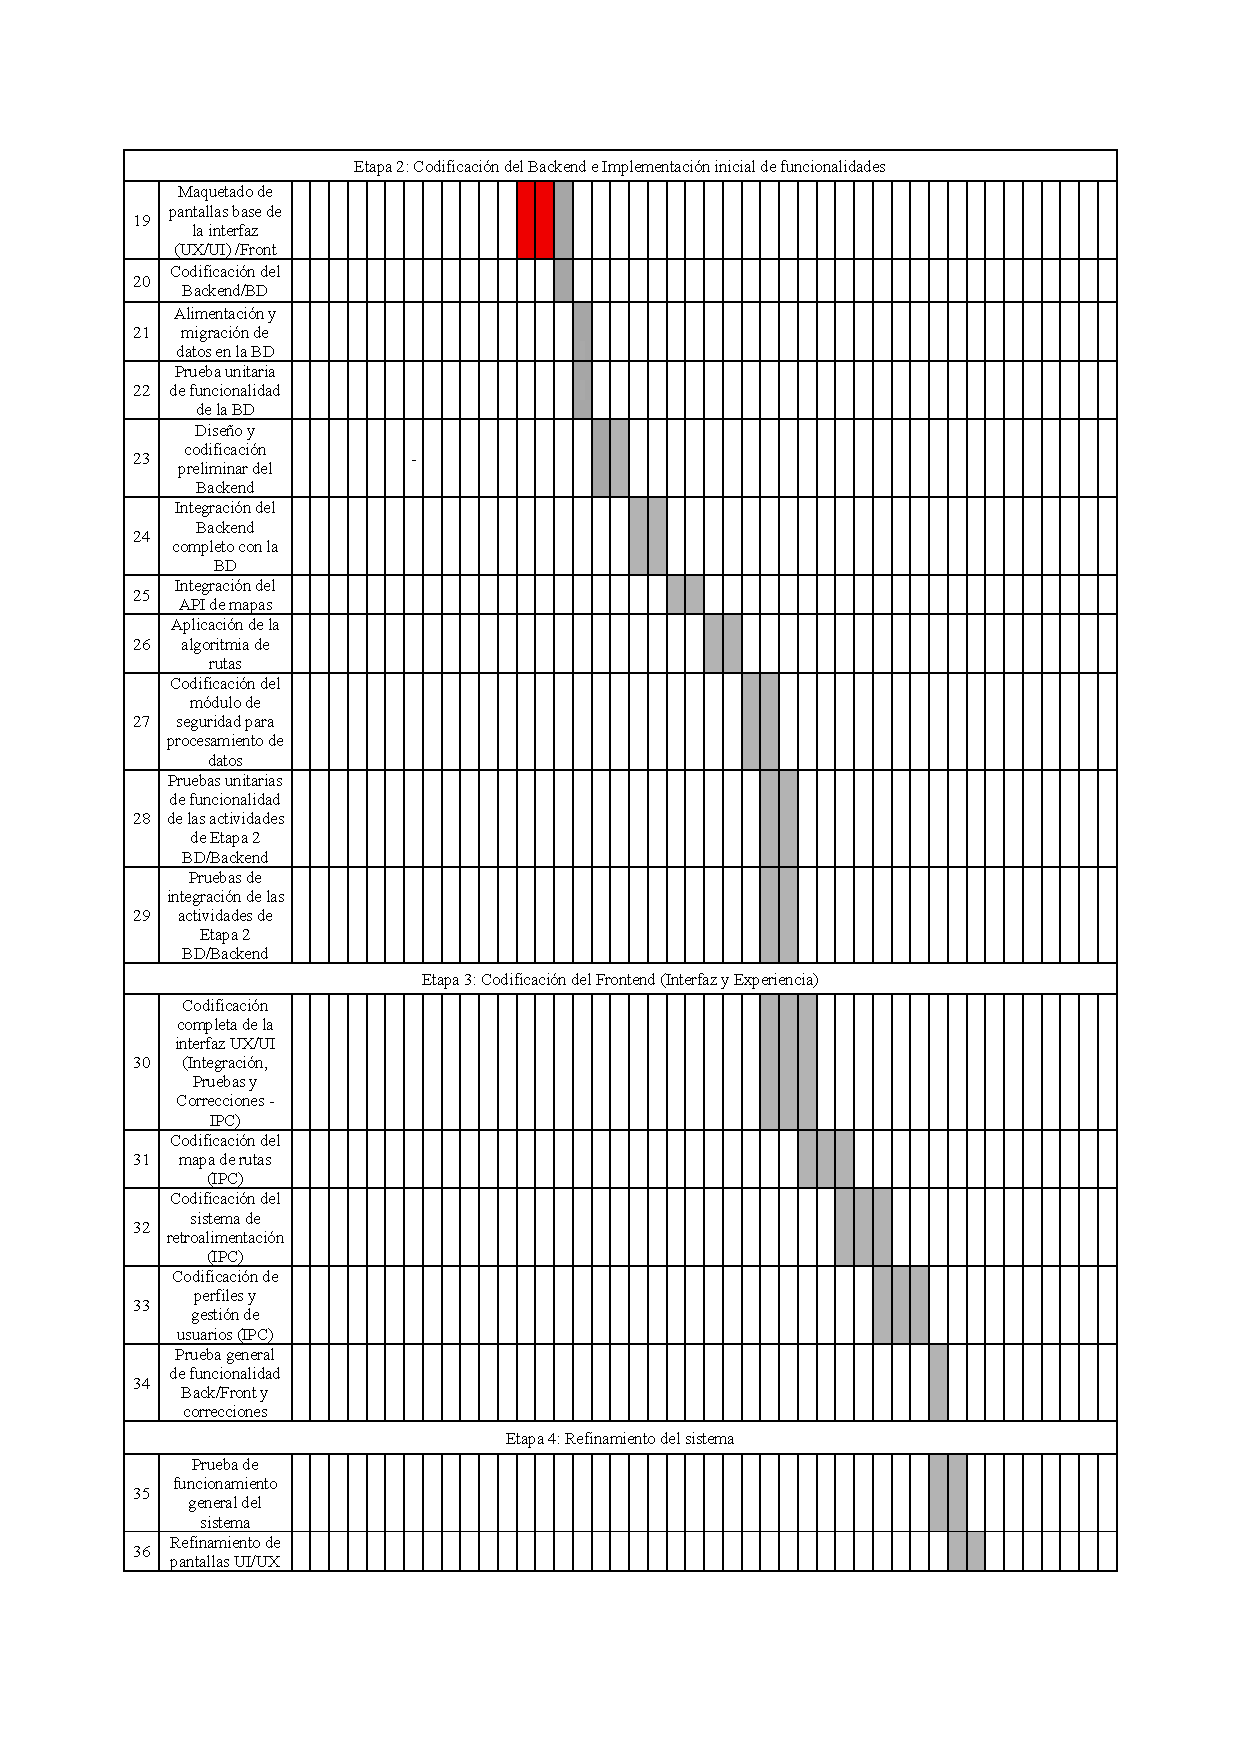
\includegraphics[width=\textwidth, trim={2cm 2cm 2cm 3cm}, clip]{figures/capitulo5_analisis_sistema/5.5_Analisis_de_Factibilidad/Cronograma_2027_TT1-1-2-2.pdf} 
    \caption*{Continuación del diagrama \ref{fig:cronograma_actividades}}
\end{figure}

\begin{figure}[H]
    \centering
    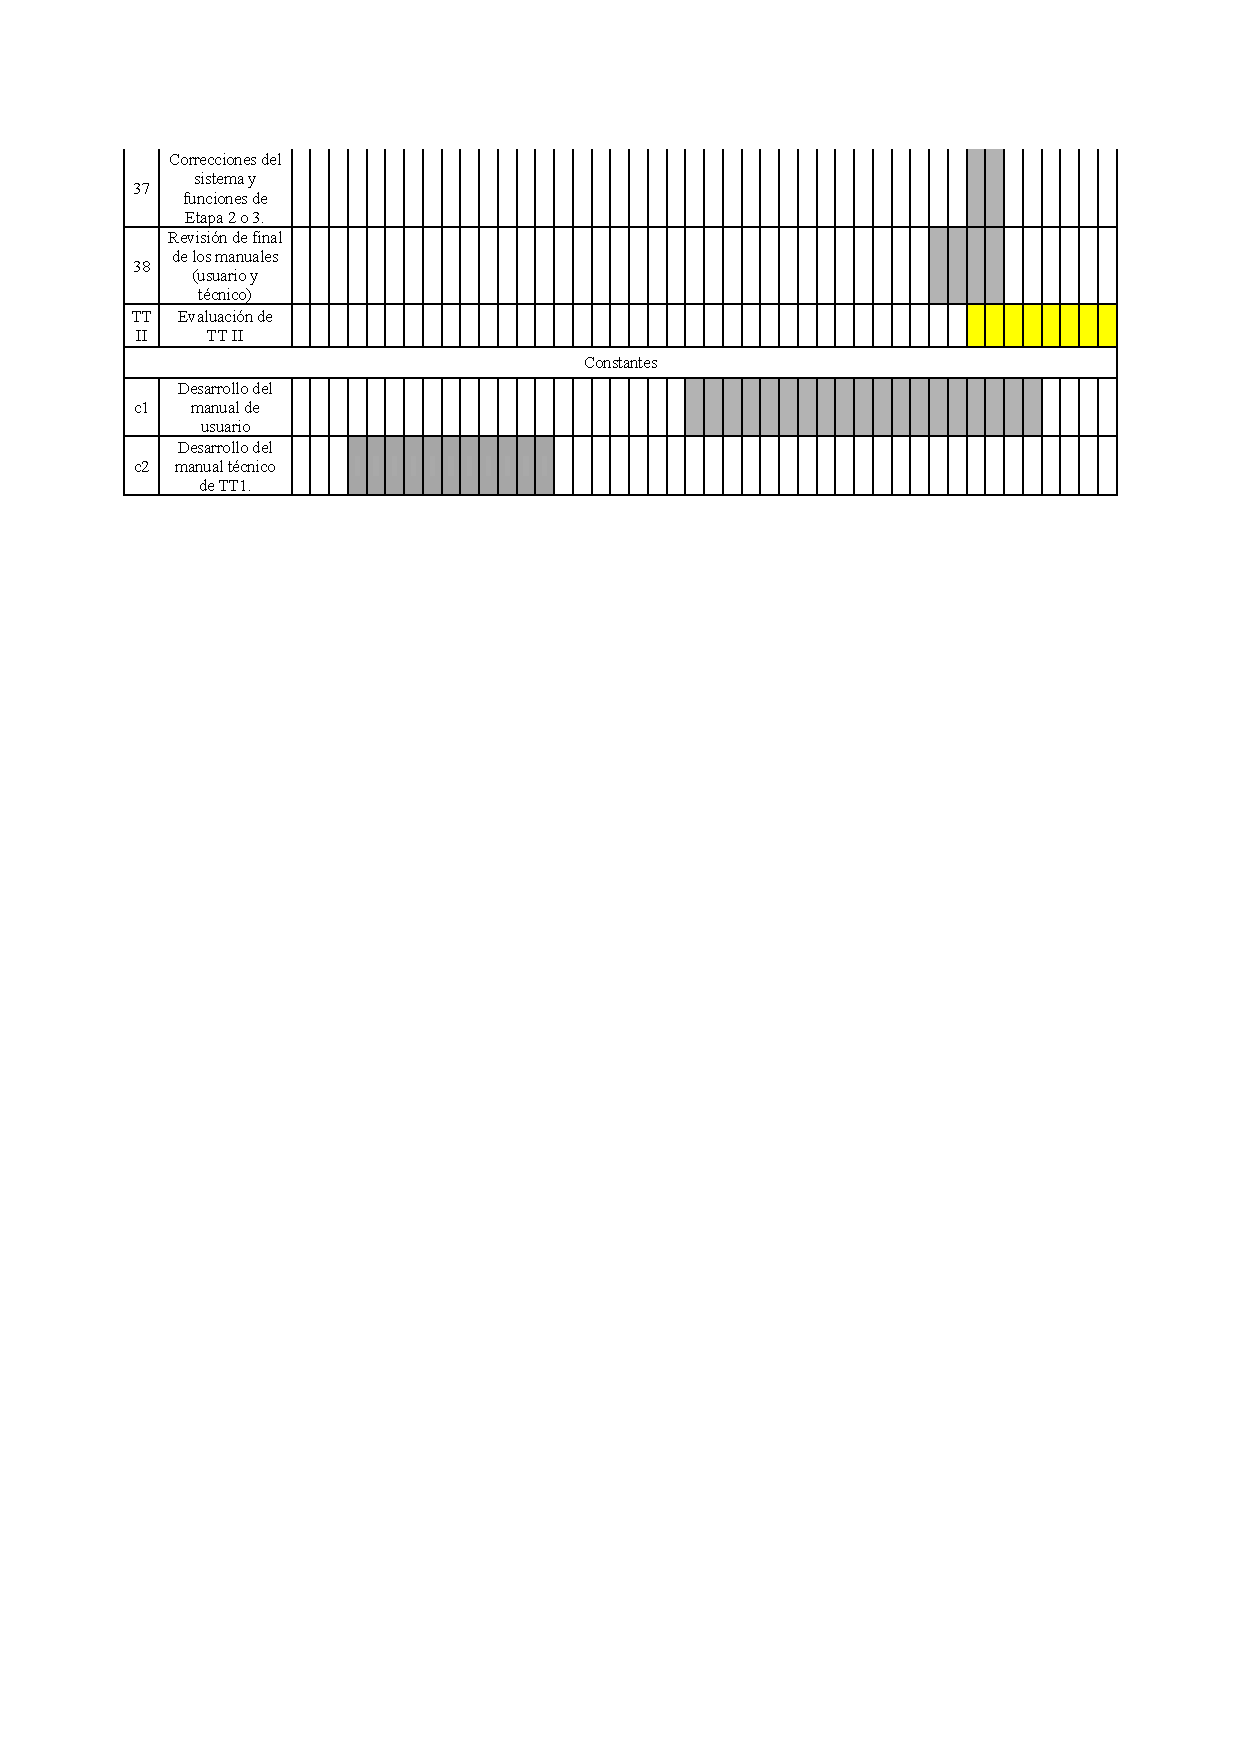
\includegraphics[width=\textwidth, trim={2cm 21cm 2cm 2cm}, clip]{figures/capitulo5_analisis_sistema/5.5_Analisis_de_Factibilidad/Cronograma_2027_TT1-3.pdf} 
    \caption*{Continuación del diagrama \ref{fig:cronograma_actividades}}
\end{figure}

Es necesario realizar la comparación entre el diagrama de Gantt (plazos definidos) contra el tiempo real requerido para el proyecto, de esta forma se observa si realmente el sistema es factible dentro de los intervalos de tiempo establecidos.

En la tabla \ref{tab:resumen_dias} se calcula el tiempo de esfuerzo requerido en base a la cantidad de horas de trabajo que el equipo invierte en el sistema obteniendo la cantidad de días laborales (tomando en cuenta una jornada de tiempo completo; 8 horas) necesarios para el desarrollo dentro del intervalo general de tiempo. 

El plazo de trabajo parte en la tercera semana de Agosto de 2026 y finaliza hasta mediados de Mayo del 2027, considerando que las fechas de presentación de TT I-II se realizan aproximadamente un mes antes de la finalización del periodo escolar. 

\begin{table}[H]
\centering
\renewcommand{\arraystretch}{1.2}
\resizebox{\textwidth}{!}{
\begin{tabular}{l c c c c c c c}
\hline
\textbf{Mes} & \textbf{Días} & \textbf{\makecell{Fin de\\semana}} & \textbf{\makecell{Días no\\laborales}} & \textbf{\makecell{Días\\hábiles}} & \textbf{\makecell{Horas de\\trabajo\\por día\\(promedio)}} & \textbf{\makecell{Horas\\totales}} & \textbf{\makecell{Días\\laborales\\(8 horas\\al día)}} \\ \hline
\textbf{Agosto} & 15 & 4 & 0 & 11 & 4 & 44 & 5.5 \\ 
\textbf{Septiembre} & 30 & 8 & 1 & 21 & 4 & 84 & 10.5 \\ 
\textbf{Octubre} & 31 & 9 & 0 & 22 & 4 & 88 & 11 \\ 
\textbf{Noviembre} & 30 & 9 & 2 & 19 & 4 & 76 & 9.5 \\ 
\textbf{Diciembre} & 30 & 8 & 0 & 22 & 4 & 88 & 11 \\ 
\textbf{Enero} & 31 & 10 & 1 & 20 & 4 & 80 & 10 \\ 
\textbf{Febrero} & 28 & 8 & 1 & 19 & 4 & 76 & 9.5 \\ 
\textbf{Marzo} & 31 & 8 & 3 & 20 & 4 & 80 & 10 \\ 
\textbf{Abril} & 30 & 8 & 5 & 17 & 4 & 68 & 8.5 \\ 
\textbf{Mayo} & 31 & 10 & 2 & 19 & 4 & 76 & 9.5 \\ 
\textbf{Junio} & 7 & 2 & 0 & 5 & 4 & 20 & 2.5 \\ \hline
\textbf{Total} & \textbf{294} & \textbf{84} & \textbf{15} & \textbf{195} & & \textbf{780} & \textbf{97.5} \\ \hline
\end{tabular}
} 
\caption{Resumen de días para el desarrollo del proyecto (Agosto 2026 - Junio 2027) con base a los plazos establecidos en el Diagrama de Gantt \ref{fig:cronograma_actividades}.}
\label{tab:resumen_dias}
\end{table}

Como se aprecia en la tabla \ref{tab:resumen_dias} se cuentan con aproximadamente 98 días laborales para el desarrollo del trabajo terminal considerando una jornada laboral de 8 días, eliminando días festivos, fines de semana y periodos que no entran en el intervalo de tiempo.

%Pendiente por desarrollar el calculo del tiempo real con formulas matematicas de cada actividad para la estimacion real de esfuerzo en tiempo requerido y el contraste con los plazos ya definidos.                                                                                                                                                                                                                            


